\documentclass[twocolumn]{ctexart}

\usepackage[utf8]{inputenc}
\usepackage[a4paper,left=0.5cm,right=0.5cm,top=1.5cm,bottom=1.5cm]{geometry}
\usepackage{multicol}
\usepackage{amsmath,amsfonts,amssymb,amsthm}
\usepackage{bm}
\usepackage{fancyhdr}
\usepackage{lastpage}
\usepackage{cite}
\usepackage{array}
\usepackage{hyperref}
\usepackage{bookmark}

\usepackage{color}

\usepackage{pgfplots}
\usepackage{tikz}

\usepackage{graphicx}

\usepackage{stfloats}%巨妈重要
\usepackage{caption}
\usepackage{float} 
\usepackage{subcaption}

\usepackage{empheq}

\pagestyle{fancy}
\setlength{\headheight}{13.0pt}

\renewcommand{\headrulewidth}{0.5pt}
\renewcommand{\footrulewidth}{0.5pt}

\renewcommand{\labelitemi}{*}

\title{\LARGE 信息光学知识点概括}
\author{\LARGE 张鑫渤 \\ {\normalsize 通讯作者:吴威圻}}
\date{\today}



\begin{document}
% \frontmatter
\twocolumn[
    \begin{@twocolumnfalse}
        \maketitle
        \thispagestyle{empty}
    \end{@twocolumnfalse}
]

\clearpage

% \twocolumn[
%     \begin{@twocolumnfalse}
%         \tableofcontents
%         \pagenumbering{Roman}
%         \thispagestyle{empty}
%     \end{@twocolumnfalse}
% ]
\tableofcontents
\pagenumbering{Roman}
\thispagestyle{empty}
\clearpage
% \mainmatter
\pagenumbering{arabic}
\section{线性系统分析}
\subsection{常用初等函数}
\subsubsection{矩形函数}
\begin{enumerate}
    \item
          函数定义:
          \begin{equation}
              rect\left(\frac{x-x_0}{a}\right)=\left\{
              \begin{aligned}
                   & 1, & \left\lvert \frac{x-x_0}{a} \right\rvert \leqslant \frac{1}{2} \\
                   & 0, & other                                                          \\
              \end{aligned}
              \right.
              \nonumber
          \end{equation}
    \item
          函数图像:
          \begin{figure}[H]
              \begin{tikzpicture}
                  [declare function={localq(\t) = (and(\t > -1/2, \t < 1/2));}]
                  \begin{axis}
                      \addplot[black,samples=200,domain=-2:2] {localq(x)} ;
                  \end{axis}
              \end{tikzpicture}
              \caption{当$x_0=0,a=1$时的$rect\left(\frac{x-x_0}{a}\right)$图像}
          \end{figure}
    \item
          作用:描述照相机快门的曝光时间,矩形孔(或狭缝)的透射系数,与某函数相乘时可限制自变量的范围,
          起到截取的作用。
    \item
          傅里叶变换函数:
          \begin{equation}
              F\left[rect\left(\frac{x}{a}\right)\right]=asinc(a\xi)
              \nonumber
          \end{equation}
\end{enumerate}

\subsubsection{sinc函数}
\begin{enumerate}
    \item
          函数定义:
          \begin{equation}
              sinc\left(\frac{x-x_0}{a}\right)=\frac{sin\pi\left(x-x_0\right)/a}{\pi\left(x-x_0\right)/a}
              \nonumber
          \end{equation}
    \item
          函数图像:
          \begin{figure}[H]
              \begin{tikzpicture}
                  [declare function={localq(\t) = (sin(deg(3.14*\t))/(deg(3.14*\t));}]
                  \begin{axis}
                      \addplot[black,samples=200] {localq(x)} ;
                  \end{axis}
              \end{tikzpicture}
              \caption{当$x_0=0,a=1$时的$sinc\left(\frac{x-x_0}{a}\right)$图像}
          \end{figure}
    \item
          作用:描述狭缝或矩形孔的夫琅禾费衍射图样。
\end{enumerate}

\subsubsection{三角函数}
\begin{enumerate}
    \item
          函数定义:
          \begin{equation}
              \Lambda\left(\frac{x}{a}\right)=\left\{
              \begin{aligned}
                   & 1-\left\lvert\frac{x}{a}\right\rvert, & \left\lvert x \right\lvert \leqslant a \\
                   & 0,                                    & other
              \end{aligned}
              \right.
              \nonumber
          \end{equation}
    \item
          函数图像:
          \begin{figure}[H]
              \begin{tikzpicture}
                  [declare function={localq(\t) = (1-abs(\t))*and(\t<1,\t>-1);}]
                  \begin{axis}
                      \addplot[black,samples=200,domain=-1.6:1.6] {localq(x)} ;
                  \end{axis}
              \end{tikzpicture}
              \caption{当$x_0=0,a=1$时的$\Lambda\left(\frac{x}{a}\right)$图像}
          \end{figure}
    \item
          作用:表示光瞳为矩形的非相干成像系统的光学传递函数。
    \item
          傅里叶变换函数:
          \begin{equation}
              F\left[ \Lambda\left(\frac{x}{a}\right) \right]=asinc^2(a\xi)
              \nonumber
          \end{equation}
\end{enumerate}

\subsubsection{符号函数}
\begin{enumerate}
    \item
          函数定义:
          \begin{equation}
              sgn\left(x\right)=\left\{
              \begin{aligned}
                   & 1,  & x>0 \\
                   & 0,  & x=0 \\
                   & -1, & x<0 \\
              \end{aligned}
              \right.
              \nonumber
          \end{equation}
    \item
          函数图像:
          \begin{figure}[H]
              \begin{tikzpicture}
                  [declare function={localq(\t) = and(\t > 0 , 1 )+and(\t < 0 , 1)*-1;}]
                  \begin{axis}
                      \addplot[black,samples=200] {localq(x)} ;
                  \end{axis}
              \end{tikzpicture}
              \caption{当$x_0=0,a=1$时的$sgn\left(x\right)$图像}
          \end{figure}
    \item
          作用:可在某处逆转某一函数的极性。
    \item
          傅里叶变换函数:
          \begin{equation}
              F\left[ sgn\left(x\right) \right]=\frac{1}{j\pi\xi}
              \nonumber
          \end{equation}
\end{enumerate}
\subsubsection{$\delta $ 函数}
\begin{enumerate}
    \item 函数定义:
          \begin{equation}
              \left.
              \begin{aligned}
                   & \delta \left( x,y \right) = \left\{
                  \begin{aligned}
                       & 0,      & x\neq0\enspace or\enspace y\neq0 \\
                       & \infty, & x=y=0
                      \nonumber
                  \end{aligned}
                  \right.                                                    \\
                   & \iint ^{\infty} _{-\infty} \delta\left(x,y\right)dxdy=1
              \end{aligned}
              \right\}
          \end{equation}
    \item
          函数图像:
          \begin{figure}[H]
              \begin{tikzpicture}
                  [declare function={localq(\t) = \t==0;}]
                  \begin{axis}
                      \addplot[black,samples=10000,domain=-0.1:0.1] {localq(x)} ;
                  \end{axis}
              \end{tikzpicture}
              \caption{当$x_0=0,a=1$时的$\delta \left( x,y \right)$图像}
          \end{figure}
    \item
          作用:描述质点、点电荷、点光源及瞬时脉冲等。其属性完全由它在积分中的作用表现出来。
    \item
          傅里叶变换函数:
          \begin{equation}
              F\left[ \delta\left(x,y\right) \right]=1
              \nonumber
          \end{equation}
\end{enumerate}

\subsubsection{梳状函数}
\begin{enumerate}
    \item
          函数定义:
          \begin{equation}
              comb\left(x\right) = \sum ^{\infty} _{n=-\infty} \delta\left(x-n\right)=\sum ^{\infty} _{-\infty} exp\left(j2\pi nx\right)
              \nonumber
          \end{equation}
    \item
          函数图像:
          \begin{figure}[H]
              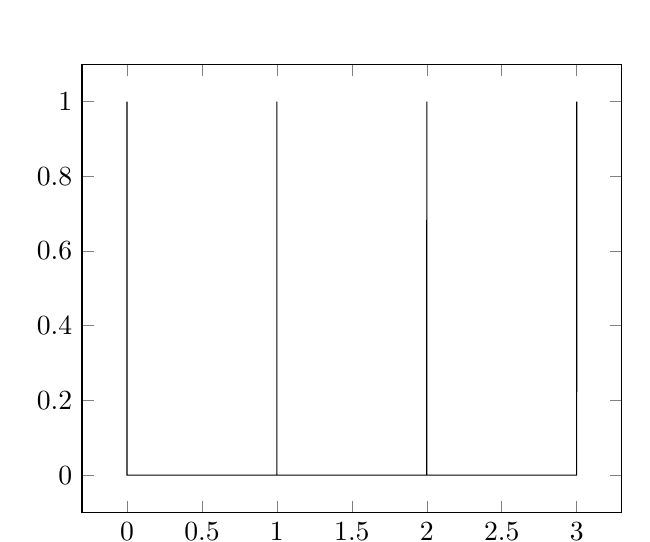
\begin{tikzpicture}
                  % [declare function={localq(\t) =exp(i*2*3.14*\t);}]
                  \begin{axis}
                      \addplot [
                          black
                      ] table [] {
                              x y
                              0 1
                              0.0001 0
                              0.9999 0
                              1 1
                              1.0001 0
                              1.9999 0
                              2 1
                              2.0001 0
                              2.9999 0
                              3 1
                          };
                  \end{axis}
              \end{tikzpicture}
              \caption{当$a=1$时的$comb\left(\frac{x}{a}\right)$图像}
          \end{figure}
    \item
          作用:可在另一函数中取样。
    \item
          傅里叶变换函数:
          \begin{equation}
              F\left[ comb\left(x,a\right) \right]=acomb\left(a\xi\right)
              \nonumber
          \end{equation}
\end{enumerate}

\subsection{二维傅里叶变换}

\subsubsection{傅里叶变换的基本性质和有关定理}
\begin{enumerate}
    \item 傅里叶正变换:
          \begin{equation}
              G\left(\xi ,\eta \right)=\iint ^{\infty} _{-\infty} g\left(x,y\right) \exp \left[-j2\pi \left(\xi x+\eta y\right)\right]\,dxdy
              \nonumber
          \end{equation}
          称为二阶傅里叶变换的核。
    \item 傅里叶反变换:
          \begin{equation}
              g\left(x ,y \right)=\iint ^{\infty} _{-\infty} G\left(\xi ,\eta \right) \exp \left[-j2\pi \left(\xi x+\eta y\right)\right]\,d\xi d\eta
              \nonumber
          \end{equation}
          ,其中$G\left(\xi ,\eta\right)$为权重因子。
    \item 性质:线性性质、对称性、迭次傅里叶变换、坐标缩放性质、平移性、体积
          对应关系和复共轭函数的傅里叶变换。
    \item 有关定理:卷积定理、相关定理、 Parseval 定理及广义 Parseval 定理等。
          \begin{equation}
              F\left[\left(x,y\right)\ast h\left(x,y\right)\right]=G\left(\xi,\eta\right) \cdot H\left(\xi ,\eta \right)
              \nonumber
          \end{equation}
\end{enumerate}
\begin{figure*}[htbp]
    \centering
    \begin{tabular}{|c|c|c|c|}
        \hline
        原函数                                                                             & 傅里叶变换函数                                                                              & 原函数                                             & 傅里叶变换函数                                                                        \\
        \hline
        1                                                                               & $\delta\left( \xi ,\eta \right)$                                                     & $rect(x)rect(y)$                                & $sinc(\xi )sinc(\eta )$                                                        \\
        \hline
        $\delta\left( x,y \right)$                                                      & $1$                                                                                  & $\Lambda (x)\Lambda (y)$                        & $sinc^2(\xi)sinc^2(\eta)$                                                      \\
        \hline
        $\delta \left(x-a,y-b \right)$                                                  & $\exp \left[-j2\pi \left(a\xi +b\eta \right)\right]$                                 & $sgn\left(x\right)sgn\left(y\right)$            & $\frac{1}{j\pi \xi}\cdot \frac{1}{j\pi \eta}$                                  \\
        \hline
        $\exp \left[-j2\pi \left(ax +by \right)\right]$                                 & $\delta\left( \xi -a,\eta -b \right)$                                                & $comb\left(x\right)comb\left(y\right)$          & $comb\left(\xi \right)comb\left(\eta \right)$                                  \\
        \hline
        $\cos \left(2\pi f_0x\right)$                                                   & $\frac{1}{2}\left[\delta \left(\xi -f_0\right)+\delta \left(\xi +f_0\right)\right]$  & $\exp \left[-\pi \left(x^2 + y^2\right)\right]$ & $\exp \left[-\pi \left(\xi ^2 + \eta ^2\right)\right]$                         \\
        \hline
        $\frac{1}{2}\left[\delta \left(x -x_0\right)+\delta \left(x +x_0\right)\right]$ & $\cos \left(2\pi \xi x_0\right)$                                                     & $circ \left(\sqrt{x^2 + y^2}\right)$            & $\frac{J_1\left(2\pi \sqrt{\xi ^2 + \eta ^2}\right)}{\sqrt{\xi ^2 + \eta ^2}}$ \\
        \hline
        $\sin \left(2\pi f_0x\right)$                                                   & $\frac{1}{2j}\left[\delta \left(\xi -f_0\right)+\delta \left(\xi +f_0\right)\right]$ & $step\left(x\right)$                            & $\frac{1}{2}\delta \left(\xi\right) +\frac{1}{j2\pi \xi}  $                    \\
        \hline
        $\frac{j}{2}\left[\delta \left(x-x_0\right)-\delta \left(x+x_0\right)\right]$   & $\sin \left(2\pi \xi x_0\right)$                                                     &                                                 &                                                                                \\
        \hline
    \end{tabular}
    \caption{常用傅里叶变换对}
\end{figure*}

\subsubsection{空间频率和空间频谱}
\begin{enumerate}
    \item $\xi =\frac{1}{X}=\frac{\cos \alpha}{\lambda},\eta =\frac{\cos \beta}{\lambda},\zeta=\frac{\cos \gamma}{\lambda},\xi ^2 +\eta ^2 +\zeta ^2 =\frac{1}{\lambda ^2}.$
          其中,$\xi ,\eta ,\zeta ,\frac{1}{\lambda}$分别是沿$X,Y,Z,K$方向的空间频率。
    \item $G\left(\xi,\eta\right)=\iint ^{\infty} _{-\infty} g\left(x,y\right)\exp \left[-j2\pi \left(\xi x+\eta y\right)\right]\,dxdy$,把$G\left(\xi ,\eta\right)$称为$g\left(x,y\right)$的空间频谱。
          写成:$G\left(\frac{\cos \alpha}{\lambda},\frac{\cos \beta}{\lambda}\right)=\iint ^{\infty} _{-\infty} g\left(x,y\right)\exp \left[-j2\pi \left(\frac{\cos \alpha}{\lambda} x+\frac{\cos \beta}{\lambda} y\right)\right]\,dxdy$,则为角谱。
\end{enumerate}

\subsubsection{傅里叶级数}
一个周期函数$f\left(t\right)$,周期$\tau=\frac{1}{v}$,它满足迪利克雷条件,即函数在一个周期内有有限个极值点和第一类间断点
(所谓第一类间断点是有函数的不连续点,在该点附近函数的值有限,其左右极限存在),则$f\left(t\right)$可展开成指数傅里叶形式
\begin{equation}
    f\left(t\right)=\frac{a_0}{2}+\sum ^\infty _{n=-\infty}C_nexp\left(j2\pi nvt \right) \nonumber
\end{equation}
其中
\begin{equation}
    C_n=\frac{1}{\tau}\int ^\tau _0 \exp\left(-j2\pi nvt\right)\,dt,\quad n=0,\pm 1,\pm 2,\cdots \nonumber
\end{equation}
由于周期函数只包含$0,\pm 1,\pm 2,\cdots$频率分量,频率的取值是离散的,所以周期函数只有离散谱。

\subsubsection{广义傅里叶变换}
广义傅里叶变换:极限意义下的傅里叶变换和$\delta $函数的傅里叶变换。

\subsection{卷积和相关}
\subsubsection{卷积}
\begin{enumerate}
    \item 二维卷积定义:
          \begin{equation}
              \begin{aligned}
                  g\left(x,y\right) & =\iint ^{\infty} _{-\infty} f\left(\alpha ,\beta\right)h\left(x-\alpha ,y-\beta \right)\,d\alpha d\beta \\
                                    & =f\left(x,y\right)\ast h\left(x,y\right)
              \end{aligned}
              \nonumber
          \end{equation}
    \item 卷积运算性质:
          \begin{enumerate}
              \item 展宽效应:
                    假如函数旨在一个有限区间内不为零,这个区间可称为函数的宽度,一般说来,卷积函数的宽度等于被卷函数宽度之和。
              \item 平滑效应:
                    被卷函数经过卷积运算,其细微结构在一定程度上被消除,函数本身的起伏震荡变得平缓圆滑,
                    在数学上有关卷积的一条定理说,在某些相当普遍的条件下,$n$个函数的卷积,当$n\to \infty$时,趋于高斯函数形式。
          \end{enumerate}
\end{enumerate}
\subsubsection{互相关、自相关的定义、物理意义}
\begin{enumerate}
    \item 互相关物理意义:互相关是两个信号之间存在多少相似性的量度。
    \item 自相关物理意义:自变量相差某一大小时,函数值间相关的量度,反映函数变化的快慢。
\end{enumerate}

\subsection{线性系统分析}
线性平移不变系统的传递函数:$H\left(\xi ,\eta \right)=\frac{G\left(\xi ,\eta \right)}{F\left(\xi ,\eta \right)}$
\subsection{二维光场分析}
平面波表达式:$A\exp \left[jk\left(x\cos \alpha +y\cos \beta\right)\right]$
\par
球面波表达式:$\frac{A}{z}\exp \left(jkz\right)\exp \left[\frac{jk}{2z}\left(x^2+y^2\right)\right]$

\section{标量衍射理论}
\subsection{标量衍射理论成立的两大条件}
\begin{enumerate}
    \item 衍射孔径比波长大得多。
    \item 观察点离衍射孔径不要太近。
\end{enumerate}

\subsection{射屏复振幅透过率}
\begin{equation}
    t\left(P\right)=\frac{U_t(P)}{U_i(P)} \nonumber
\end{equation}
或是以一定形式限制波面范围或使振幅以一定分布衰减,或是以一定的空间分布使相位延迟,
或是两者兼而有之,都会引起衍射。
\subsection{惠更斯——菲涅耳原理}
\begin{equation}
    U\left(Q\right)=c\iint _{\Sigma} U_0\left(P\right)K\left(\theta \right)\frac{\exp \left(jkr\right)}{r}\,ds \nonumber
\end{equation}
\subsection{基尔霍夫衍射理论}
\begin{equation}
    \begin{aligned}
        U\left(Q\right)= & \frac{1}{j\lambda}\iint _{\Sigma} \frac{a_0\exp (jkr_0)}{r_0}\cdot                                                                        \\
                         & \left[\frac{\cos \left(\vec{n},\vec{r}\right)}{2}-\frac{\cos \left(\vec{n},\vec{r_0}\right)}{2}\right]\frac{\exp \left(jkr\right)}{r}\,ds
    \end{aligned}
    \nonumber
\end{equation}
$h\left(P,Q\right)=\frac{1}{j\lambda}\frac{\exp \left(jkr\right)}{r}K\left(\theta \right)$脉冲响应或点扩散函数。
所以:$U\left(Q\right)=\iint U_0(P)h\left(P,Q\right)\,ds$。\\
当光源足够远,且入射光在孔径平面上各点的入射角都不大时,
$\because \cos \left(\vec{n},\vec{r_0}\right)\approx -1,\cos \left(\vec{n},\vec{r}\right)\approx 1$\\
$\therefore K\left(\theta \right)\approx 1$\\
故$h\left(P,Q\right)=\frac{1}{j\lambda}\frac{\exp \left(jkr\right)}{z},r\approx z\left\{1+\frac{1}{2}\left[\left(\frac{x-x_0}{z}\right)^2+\left(\frac{y-y_0}{z}\right)^2\right]\right\}$

\subsection{菲涅耳衍射——近场衍射}
条件:$\frac{2\pi}{\lambda}\frac{\left[\left(x-x_0\right)^2+\left(y-y_0\right)^2\right]_{max}}{8z^3}\ll 2\pi$。其脉冲相应具有空不变的形式。
\begin{equation}
    \begin{aligned}
        U\left(x,y\right)=\frac{\exp \left(jkz\right)}{j\lambda z} & \exp \left[\frac{jk}{2z}\left(x^2+y^2\right)\right]\iint ^{\infty} _{-\infty}U_0\left(x_0,y_0\right)\cdot \\
                                                                   & \exp \left[\frac{jk}{2z}\left(x_0^2+y_0^2\right)\right]\cdot                                              \\
                                                                   & \exp \left[\frac{-j2\pi}{\lambda z}\left(xx_0+yy_0\right)\right]\,dx_0dy_0
    \end{aligned}
    \nonumber
\end{equation}
\subsection{夫琅禾费衍射——远场衍射}
条件:$\frac{2\pi}{\lambda}\frac{\left(x_0^2+y_0^2\right)_{max}}{2z}\ll 2\pi$。其脉冲相应不再具有空不变的形式。
\begin{equation}
    \begin{aligned}
        U\left(x,y\right)=\frac{\exp \left(jkz\right)}{j\lambda z} & \exp \left[\frac{jk}{2z}\left(x^2+y^2\right)\right]\iint ^\infty _{-\infty} U_0\left(x_0,y_0\right)\cdot \\
                                                                   & \exp \left[-j\frac{2\pi}{\lambda z}\left(xx_0+yy_0\right)\right]\,dx_0dy_0
    \end{aligned}
    \nonumber
\end{equation}
\subsection{夫琅禾费衍射的条件及与菲涅耳衍射之比较}
\begin{enumerate}
    \item 菲涅耳衍射的复振幅分布正比于
    \begin{equation}
        U_0\left(x_0,y_0\right)\exp \left[\frac{jk}{2z}\left(x_0^2+y_0^2\right)\right]
        \nonumber
    \end{equation}
    的傅里叶变换,因此随着距离 $z$ 的增大,观察平面上衍射光场分布会发生变化,
    仅就轴上点,而言,随着距离 $z$ 的变化其亮暗是交替变化
    \item 夫琅禾费衍射的复振幅分布正比于 $U_0\left(x_0,y_0\right)$的傅里叶变换,当 $z$ 变化时,
    衍射图样只是按比例放大或缩小,图样形状不会发生变化。
\end{enumerate}
\subsection{衍射的角谱理论}
\begin{enumerate}
    \item 角谱的传播:
    \begin{equation}
        \begin{aligned}
            A\left(\frac{\cos \alpha}{\lambda},\frac{\cos \beta}{\lambda}\right)=&A_0\left(\frac{\cos \alpha}{\lambda},\frac{\cos \beta}{\lambda}\right)\cdot\\
            &\exp \left(jkz\sqrt{1-\cos ^2 \alpha -\cos ^2 \beta}\right),\\
            H\left(\xi ,\eta \right)=&\frac{A\left(\xi ,\eta\right)}{A_0\left(\xi ,\eta\right)}\\
            =&\exp \left[jk\cdot z\sqrt{1-\left(\lambda \xi\right)^2-\left(\lambda \eta\right)^2}\right]
        \end{aligned}
        \nonumber
    \end{equation}
    即:\par
    基尔霍夫理论是描述球面子波相干叠加的理论,它在空域讨论光的传播。
    角谱理论是衍射的平面波理论,它在频域讨论光的传播。
    \item 孔径对角谱的影响:
    \begin{equation}
        \begin{aligned}
            A_o\left(\frac{\cos \alpha}{\lambda},\frac{\cos \beta}{\lambda}\right)=&A_i\left(\frac{\cos \alpha}{\lambda},\frac{\cos \beta}{\lambda}\right)\\
            \ast& T\left(\frac{\cos \alpha}{\lambda},\frac{\cos \beta}{\lambda}\right)
        \end{aligned}
        \nonumber
    \end{equation}
    衍射孔径展宽了角谱,孔径越小,角谱越宽。从空域看,
    孔径的作用限制了入射球面波的大小,从频域看,则是展宽了入射光场的角谱。
\end{enumerate}

\subsection{透镜的傅里叶变换性}
\subsubsection{孔径函数}
\begin{equation}
    \begin{aligned}
        t\left(x,y\right)=P\left(x,y\right)\exp \left[-j\frac{k}{2f}\left(x^2+y^2\right)\right]
    \end{aligned}
    \nonumber
\end{equation}
\begin{enumerate}
    \item 相位变换作用:$t\left(x,y\right)=p\left(x,y\right)\exp \left[-\frac{jk}{2f}\left(x^2+y^2\right)\right]$。
    \item 透镜的傅里叶变换性:\begin{enumerate}
        \item 物在透镜前时,仅在前焦平面处无二次位相因子。
        \item 物在透镜后时,均有二次位相因子。
    \end{enumerate}
\end{enumerate}


\section{光学成像系统的传递函数}
几何光学:空域研究成像规律,采用星点法和分辨率法(像质评价)。\\
信息光学:频域研究成像规律,采用光学传递函数法(全面、科学像质评价)。
\subsection{透镜的点扩散函数}
当该面元的光振动为单位脉冲即$\delta$函数时,这个像场分布函数叫做点扩散函数或脉冲相应。
通常用$h\left(x_o,y_o;x_i,y_i\right)$表示。\par
当透镜的孔径比较大时,物面上每一物点产生的脉冲响应是一个很小的像斑,那么能够对于
泉面上$(x_i,y_i)$点光场产生有意义贡献的,必定是物面上以几何成像所对应的以物点为中心的微小区域。
在这个区域内可近似地认为$x_o,y_o$不变,其值与$(x_i,y_i)$点的共轭物坐标$x_o=x_i/M,y_o=y_i/M$相同,
即可作以下近似:\begin{equation}
    \exp\left[j\frac{k}{2d_o}\left(x_o^2+y_o^2\right) \right]\approx \exp \left[j\frac{k}{2d_o}\left(\frac{x_i^2+y_i^2}{M^2}\right)\right]
    \nonumber
\end{equation}
这样一来,点扩散函数的形式为\begin{equation}
    \begin{aligned}
        h&\left(x_o,y_o;x_i,y_i\right)=\frac{1}{\lambda ^2d_o d_i}\iint ^\infty _{-\infty} P\left(x,y\right)\\
        &\exp \left\{-jk\left[\left(\frac{x_i}{d_i}+\frac{x_o}{d_o}\right)x+\left(\frac{y_i}{d_i}+\frac{y_o}{d_o}\right)y\right]\right\}\,dxdy
    \end{aligned}
    \nonumber
\end{equation}

\subsection{衍射受限系统的点扩散函数}
\begin{equation}
    \begin{aligned}
        &h\left(x_i-\tilde{x_0},y_i-\tilde{y_0}\right)=K\lambda ^2 d ^2 _i \iint ^\infty _{-\infty}P\left(\lambda d_i\tilde{x},\lambda d_i\tilde{y}\right)\cdot       \\
        &\exp \left\{-j2\pi \left[\left(x_i-\tilde{x_0}\right)\tilde{x}+\left(y_i-\tilde{y_0}\right)\tilde{y}\right]\right\}\,d\tilde{x}d\tilde{y}
    \end{aligned}
    \nonumber
\end{equation}
光瞳相对于$\lambda d_i$足够大时:\\
$h\left(x_i-\tilde{x_o},y_i-\tilde{y_o}\right)\cong K\lambda ^2 d_i^2\delta \left(x_i-\tilde{x_o},y_i-\tilde{y_o}\right)$\\
理想情况:点物成点像。
\subsection{相干照明下衍射受限系统的成像规律}
\begin{equation}
    U_i\left(x_i,y_i\right)=\tilde{h}\left(x_i,y_i\right)\ast U_g\left(x_i,y_i\right)
    \nonumber
\end{equation}
其中,$\tilde{h}\left(x_i,y_i\right)=F\left[P\left(\lambda d_i \tilde{x},\lambda d_i \tilde{y}\right)\right]$,\\
$U_g\left(x_i,y_i\right)=\frac{1}{M}U_0\left(\frac{x_i}{M},\frac{y_i}{M}\right)$为理想像。\par
表明:物$U_0\left(x_0,y_0\right)$通过衍射受限系统后的像$U_i\left(x_i,y_i\right)$是$U_0\left(x_0,y_0\right)$的理想像
$U_g\left(x_i,y_i\right)$和点扩散函数$\tilde{h}\left(x_i,y_i\right)$的卷积。\par
可见,在相干照明条件下,对于衍射受限成像系统,表征成像系统特征的点扩散函数$\tilde{h}$,
仅决定于系统的光瞳函数$P$,可见,光曈函数对于与衍射受限系统成像的重要。
\subsection{颜色和受限系统的相干传递函数}
\begin{equation}
    H\left(\xi ,\eta \right)=P\left(\lambda d_i \xi , \lambda d_i \eta\right)
    \nonumber
\end{equation}

\subsection{截止频率}
衍射受限系统是一个低通滤波器,低于某一频率的指数基元成分将按原样通过,
高于该频率的指数基元成分将被截止,这个特征频率称为系统的截止频率。\\
注意:渐晕效应。
\begin{enumerate}
    \item 圆形光瞳:$\rho _c =\frac{D}{2\lambda d_i},\rho _{oc}=M\rho _c=\frac{D}{2\lambda d_o} $
    \item 正方形光瞳不同方向的截止频率不同,$45^\circ$方向最大$\rho _{cmax}=\frac{\sqrt{2}a}{2\lambda d_i}$
    \item 长方形光瞳不同方向的频率不同,对角线方向最大$\rho _{cmax}=\frac{\sqrt{a^2+b^2}}{2\lambda d_i}$。
\end{enumerate}

\section{光学全息}
\subsection{普通照相与全息照相的比较(定义)}
普通照相是根据几何光学成像原理,记录下光波的强度(即振幅),而全息
照相是根据波动光学干涉、衍射原理,能记录光波的振幅和相位(完全信息)。
\subsection{全息照相的核心}
波前记录(干涉)和再现(衍射)。\par
参考光波一般选用比较简单的平面波或球面波,且参考光波通常比物光波强的多。
\begin{enumerate}
    \item 方法:干涉法(标准方法,即将空间相位调制→空间强度调制)。
    \item 特点:全息图实际上就是一幅干涉图。
    \item 记录过程的线性条件:把曝光期间内的入射光强线性地变换为显影后的负片的振幅透过率。
    \item 分类:\begin{enumerate}
        \item 物、参位置:同轴全息+离轴全息。
        \item 物、图位置:菲涅耳全息图+像面全息图+傅里叶变换全息图。
        \item 介质厚度:平面全息图+体积全息图。
    \end{enumerate}
\end{enumerate}
\subsection{全息基本公式}
\begin{equation}
    \begin{aligned}
        &\left(t_b+\beta ^\prime O^2\right)Ce^{j\delta _C}&+ORCe^{j\left(\delta _O-\delta _r +\delta _C\right)}+&ORCe^{-j\left(\delta _O - \delta _r - \delta _C\right)}\\
       &\text{0级(背景光)}    &\text{+1级(虚像)}    &\text{-1级(实像)}
    \end{aligned}
    \nonumber
\end{equation}
\subsection{菲涅尔全息图}
直接记录物体光波本身,不需透镜。记录介质与物体距离满足 $Fresnel$ 衍射条件。\\
像位置坐标:
\begin{equation}
    \begin{aligned}
        &z_i=\left(\frac{1}{z_p}\pm \frac{\lambda _2}{\lambda _1 z_r}\mp \frac{\lambda_2}{\lambda_1z_o}\right)^{-1}\\
        &x_i=\mp\frac{\lambda _2 z_i}{\lambda _1 z_o}x_o \pm \frac{\lambda _2 z_i}{\lambda _1 z_r}x_r+\frac{z_i}{z_p}x_p,\\
        &y_i=\mp\frac{\lambda _2 z_i}{\lambda _1 z_o}y_o \pm \frac{\lambda _2 z_i}{\lambda _1 z_r}y_r+\frac{z_i}{z_p}y_p
    \end{aligned}
    \nonumber
\end{equation}
横向放大率:$M=\left\lvert \frac{dx_i}{dx_o}\right\lvert =\left\lvert \frac{dy_i}{dy_o}\right\lvert=\left\lvert \frac{\lambda _2 z_i}{\lambda _1 z_o}\right\lvert=\left\lvert 1-\frac{z_0}{z_r}\mp \frac{\lambda ^2 z_o}{\lambda _1 z_p}\right\lvert ^{-1}$
Information Optics.pdf纵向放大率:$M_z=\left\lvert \frac{dz_i}{dz_o}\right\lvert=\frac{\lambda _1}{\lambda _2}M^2$
$z_i$为正时,乃发散球面波,再现像是虚像。$z_i$为负时,乃会聚球面波,再现像是实像。
\subsection{傅里叶变换全息图}
\begin{enumerate}
    \item 定义:物体或图像频谱的全息记录。
    \item 特点:不是记录物光波本身,而是记录物光波的傅里叶变换。
    \item 照明方式:平行光照明和点光源照明,相互是独立的。
\end{enumerate}

\subsection{位相全息图}
\begin{enumerate}
    \item 定义:照明光波通过全息图时,受到均匀吸收,仅仅是相位被调制。
    \item 两种制作方法:表面浮雕型和折射率型。记录物质的厚度改变,折射率不变。改变记录物质的折射率,不改变折射率。
    \item 性质:在线性记录条件下,相位变化与曝光光强成正比。
\end{enumerate}

\subsection{平面全息图的衍射效率}
\begin{enumerate}
    \item 定义:全息图的一级衍射成像光通量与照明全息图的总光通量之比。
    \item 振幅全息图的衍射效率:正弦型(6.25\%), 矩形(10.13\%)
    \item 位相全息图的衍射效率:正弦型(33.9\%), 矩形(40.4\%)
\end{enumerate}
结论:无论振幅型还是位相型,矩形波衍射效率均大于正弦波。

\section{空间滤波}
\subsection{阿贝成像理论}
第 1 步:物体($P_1$)经 $L$ 在透镜后焦面($P_2$)成各级衍射斑(分频)。\par
第 2 步:各级衍射斑在像面($P_3$)相互干涉成像(合成)。
\subsection{空间滤波的傅里叶分析}
透镜作频谱分析器,空间滤波器改变物体光的频谱。
\subsection{空间滤波系统}
经典的$4f$系统(尚有其他三种系统)。
\subsection{空间滤波器}
位于空间频谱平面上的一种模片,它改变输入信息的空间频谱,
从而实现对输入信息的某种变换。分类:\par
\begin{enumerate}
    \item 二元振幅滤波器。
    \item 振幅滤波器。
    \item 相位滤波器。
    \item 复数滤波器。
\end{enumerate}
二元振幅滤波器亦可分为:
\begin{enumerate}
    \item 低通滤波器。
    \item 高通滤波器。
    \item 带通滤波器。
    \item 方向滤波器。
\end{enumerate}
\subsection{空间滤波应用}
\begin{enumerate}
    \item 策尼克相衬显微镜:在频谱面上改变中心相位$\pm \pi/2$,
    强度变化与位相变化成线性关系$I=1\pm 2\varphi$且变化的幅度相对背景而言加倍。
    $+$:正相衬;$-$:负相衬。
    \item 补偿滤波器:为补偿离焦成像系统的缺陷,可采用组合滤波器可改善图像
    质量。其吸引板可衰减传递函数 H 低频峰值,提高像的对比,突出细节;相移
    板可使传递函数 $H$ 的第一个负瓣相移$\pi$纠正对比反转。
    \item $\theta$调制技术:利用光栅与其谱点的对应关系来改变光栅像,
    将原始像$f_o\left(x_0,y_0\right)$ 变成按一定角度$\theta$的光栅调制的像$f^\prime_m\left(x^\prime _0,y^\prime _0\right)$。
    $\theta$角的大小与物体振幅分割的等级个数$m$的大小有关(一般$\theta = 180 m$)。
\end{enumerate}

\section{相干光学处理}
\subsection{光学信息处理的分类}
\begin{enumerate}
    \item 从物像关系或者输入和输出的关系来说
    \begin{enumerate}
        \item 线性处理与非线性处理
        \item 空间不变与空间变处理
    \end{enumerate}
    \item 从所使用光源的空间和时间相干性来说
    \begin{enumerate}
        \item 相干光处理
        \item 非相干光处理
        \item 白光光学处理
    \end{enumerate}
\end{enumerate}
\subsection{光学信息处理内容}
\begin{enumerate}
    \item 光学图像识别(匹配滤波)
    \item 图像相加(代数运算)
    \item 图像相减(代数运算)
    \item 图像边缘(高通滤波)
    \item 图像消模糊(逆滤波器和维纳滤波器)
\end{enumerate}
\subsection{图像相减作用}
用于检测两张近似图像之间的差异,使我们能研究事物的变化。\\
方法:光栅编码(空域编码频域解码相减)和光栅衍射(正弦光栅滤波器相减)。
\subsection{匹配空间滤波器}
\begin{enumerate}
    \item 所谓“匹配”,实质上是在频域对输入信号频谱的相位进行补偿,形成平面相位分布。
    \item 匹配空间滤波器在光学特征识别中起重要作用。
    \item 匹配滤波器是复数滤波器,可用光学全息或计算全息的方法制作。
\end{enumerate}

\subsection{图像识别}
采用匹配滤波进行相关检测是图像识别的一种重要手段。\\
联合变换相关识别:在输出平面得到目标图像与参考图像的相关输出。
还用于指纹和汉字手写体的实时识别。

\subsection{不变的图样识别光学方法}
使光学相关识别系统具有“不变应万变”的鲁棒性,
降低或消除对诸如尺寸大小和旋转等额外参数的敏感程度,常用的解决方法有:
\begin{enumerate}
    \item 梅林相关器:对物体放大率具有某种不变性。
    \item 圆谐波相关:能很好地解决物体的旋转不变性问题。
    \item 合成判别式函数:用来制作单个的图样识别滤波器,相关性质是某一组训
    练图像预先制作的,这些图像与参考滤波器之间所需的相关性质事先已经知道。
\end{enumerate}

\subsection{模糊图像的复原}
原因:传递函数的缺陷。\par
方法:逆滤波器(解卷积)和维纳滤波器(最小均方误差滤波器)。
\end{document}